\setAuthor{Jaan Kalda}
\setRound{piirkonnavoor}
\setYear{2009}
\setNumber{G 6}
\setDifficulty{6}
\setTopic{Elektrostaatika}

\prob{Liikuv laeng}
Laetud osake laengu ja massi suhtega $q/m = \SI{1}{C/kg}$ seisab algselt paigal. Seejärel hakkab ta liikuma $x$- ja $y$-telje sihis
toimivate elektrivälja impulsside mõjul. Elektrivälja vastavate komponentide $E_x$ ja $E_y$ sõltuvus ajast on toodud graafikul (graafiku mastaap
ei ole korrektne, juhenduda tuleb graafikul näidatud numbritest impulsi
kestvuse $\tau = \SI{1}{ms}$ ja amplituudi $E_0 = \SI{1}{kV/m}$ ning perioodi $T = \SI{2}{s}$
jaoks). Visandage osakese trajektoor ja leidke keskmine kiirus (visandi tegemisel ja arvutustes võib lugeda ajavahemiku $\tau = \SI{1}{ms}$ jooksul
toimuvad muutused hetkelisteks). 

\begin{center}
	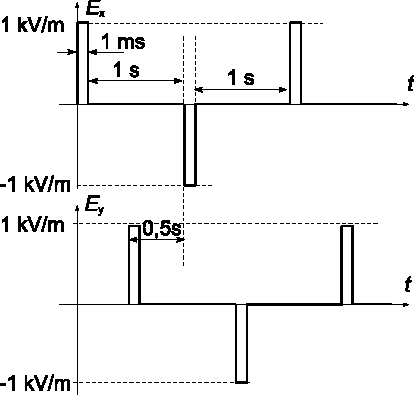
\includegraphics[width=0.6\linewidth]{2009-v2g-06-yl}
\end{center}

\hint
Osakese asukohta on mugavam leida vaadeldes eraldi osakese $x$- ja $y$-koordinaate. Laengu keskmine kiirus on leitav perioodi jooksul sooritatud nihke ja perioodi suhtena.

\solu
Esimene impulss annab alguses laengule $x$-suunalise impulsi $mv_x = qE_x\tau$ , millest
\[
v_{x}=\frac{q}{m} E_{x} \tau= \SI{1}{m/s}.
\]
Ajavahemiku $t_1 = T /4$ jooksul kuni järgmise impulsini jõuab osake liikuda sirgjooneliselt piki $x$-telge kaugusele
$s_x = v_xT /4 = \SI{0,5}{m}$. Seejärel saab ta impulsi y-telje sihis, mistõttu omandab ka kiiruse $y$-komponent
samasuguse väärtuse: $v_y = v_x = \SI{1}{m/s}$, mistõttu ta liigub \num{45}-kraadise nurga all,
sooritades kuni järgmise impulsini nii $x$- kui $y$-telje sihis nihke $s_x = s_y = \SI{0,5}{m}$. Järgmine impulss peatab $x$-telje sihilise (kuid muutmata $y$-sihilist) liikumise, nii et
osake nihkub nüüd piki $y$-telge kaugusele $s_y = \SI{0,5}{m}$. Järgmine impulss peatab ka $x$-suunalise liikumise, nii et osake jääb paigale. Edasi kordub protsess otsast
peale. Eelpooltoodud tulemuste põhjal saame juuresoleva trajektoori.

\begin{center}
	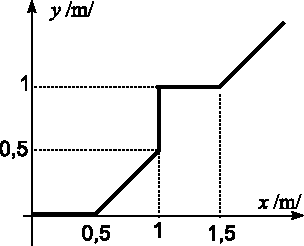
\includegraphics[width=0.6\linewidth]{2009-v2g-06-lah}
\end{center}

Keskmise kiiruse leiame perioodi jooksul sooritatud nihke $s = \sqrt{1+1}\si{m}$ perioodi $T = \SI{2}{s}$ suhtena, $v \approx \SI{0,7}{m/s}$ .
\probend